\clearpage

\appendix

\section{Partial derivatives of sample statistics}

We derive below the partial derivatives of common sample statistics for a
dataset \(x = \{x_1, x_2, \ldots, x_n\}\) with respect to an individual
observation \(x_i\), where \(n\) denotes the sample size. The Kronecker delta
\(\delta_{ij}\) equals 1 when \(i = j\) and 0 otherwise.

\subsection{Sample Mean}
\label{sec:sample_mean_derivation}

The partial derivative of the sample mean with respect to \(x_i\) is constant:
\begin{equation}
    \frac{\partial \overline{x}}{\partial x_i} = \frac{1}{n}.
    \label{eq:sample_mean_derivative}
\end{equation}

\begin{proof}
    The sample mean is defined as
    \[
        \overline{x} = \frac{1}{n} \sum_{j=1}^{n} x_j.
    \]
    Taking the partial derivative with respect to \(x_i\) gives
    \[
        \frac{\partial \overline{x}}{\partial x_i}
        = \frac{\partial}{\partial x_i} \left( \frac{1}{n} \sum_{j=1}^{n} x_j \right)
        = \frac{1}{n} \sum_{j=1}^{n} \frac{\partial x_j}{\partial x_i}
        = \frac{1}{n} \sum_{j=1}^{n} \delta_{ij}
        = \frac{1}{n}.
    \]
\end{proof}

\subsection{Sample Variance}
\label{sec:sample_variance_derivation}

The partial derivative of the sample variance with respect to \(x_i\) is
\begin{equation}
    \frac{\partial s^2}{\partial x_i} = \frac{2(x_i - \overline{x})}{n-1}.
    \label{eq:sample_variance_derivative}
\end{equation}

\begin{proof}
    The sample variance is defined as
    \[
        s^2 = \frac{1}{n-1} \sum_{j=1}^{n} {(x_j - \overline{x})}^2.
    \]
    Differentiating with respect to \(x_i\) yields
    \begin{align*}
        \frac{\partial s^2}{\partial x_i}
         & = \frac{1}{n-1} \sum_{j=1}^{n}
        \frac{\partial}{\partial x_i} (x_j - \overline{x})^2                           \\
         & = \frac{2}{n-1} \sum_{j=1}^{n}
        (x_j - \overline{x}) \frac{\partial (x_j - \overline{x})}{\partial x_i}        \\
         & = \frac{2}{n-1} \sum_{j=1}^{n}
        (x_j - \overline{x}) \left( \delta_{ij} - \frac{1}{n} \right)                  \\
         & = \frac{2}{n-1} \left[ (x_i - \overline{x})\!\left( 1 - \frac{1}{n} \right)
        - \frac{1}{n} \sum_{\substack{j=1                                              \\ j \ne i}}^{n} (x_j - \overline{x}) \right].
    \end{align*}
    Since \(\sum_{j=1}^{n} (x_j - \overline{x}) = 0\) then \(\sum_{\substack{j=1 \\ j \ne i}}^{n} (x_j - \overline{x}) = - (x_i - \overline{x})\) so the second term simplifies, giving
    \[
        \frac{\partial s^2}{\partial x_i}
        = \frac{2(x_i - \overline{x})}{n-1}.
    \]
\end{proof}

\subsection{Sample Standard Deviation}
\label{sec:sample_std_derivation}

The partial derivative of the sample standard deviation with respect to \(x_i\)
is
\begin{equation}
    \frac{\partial s}{\partial x_i} = \frac{x_i - \overline{x}}{(n-1)s}.
    \label{eq:sample_std_derivative}
\end{equation}

\begin{proof}
    Given that \(s = \sqrt{s^2}\), the derivative follows directly from the chain rule:
    \begin{align*}
        \frac{\partial s^2}{\partial x_i}  & = \frac{2(x_i - \overline{x})}{n-1}, \\
        2s \frac{\partial s}{\partial x_i} & = \frac{2(x_i - \overline{x})}{n-1}, \\
        \frac{\partial s}{\partial x_i}    & = \frac{x_i - \overline{x}}{(n-1)s}.
    \end{align*}
\end{proof}

\subsection{Pooled Standard Deviation}
\label{sec:pooled_std_derivation}

The pooled standard deviation is a weighted average of the variances of two
groups \(|G_1|=n_1\) and \(|G_2|=n_2\) with \(df=n_1+n_2-2\). Its partial
derivative with respect to \(x_i\), \(i \in G_g\) is given by
\begin{equation}
    \frac{\partial s_p}{\partial x_i} = \frac{x_i - \overline{x}_g}{df s_p}.
\end{equation}

\begin{proof}
    Let \(x\) be partitioned into two groups \(G_1\) and \(G_2\) with sizes \(n_1\)
    and \(n_2\), \(\overline{x}_1\), \(\overline{x}_2\) be the sample means and
    \(s_1\), \(s_2\) be the sample standard deviations of groups \(G_1\) and
    \(G_2\), respectively. Let \(df=n_1+n_2-2\) then the pooled standard deviation \(s_p\) is defined as
    \[
        s_p = \sqrt{\frac{(n_1 - 1)s_1^2 + (n_2 - 1)s_2^2}{df}}.
    \]
    Differentiating \(s_p\) with respect to \(x_i\) in group \(G_g\) gives:
    \begin{align*}
        \frac{\partial s_p}{\partial x_i} & = \frac{\partial}{\partial x_i} {\left[\frac{(n_1 - 1)s_1^2 + (n_2 - 1)s_2^2}{df}\right]}^{\frac{1}{2}}   \\
                                          & = \frac{1}{2 s_p} \frac{1}{df} \frac{\partial}{\partial x_i} \left[(n_1 - 1)s_1^2 + (n_2 - 1)s_2^2\right] \\
                                          & = \frac{1}{df}\frac{1}{2 s_p}2(x_i - \bar{x}_g)                                                           \\
        \frac{\partial s_p}{\partial x_i} & = \frac{x_i - \bar{x}_g}{df s_p}
    \end{align*}
\end{proof}

\subsection{Sample Covariance}
\label{sec:sample_covariance_derivation}

The partial derivative of the sample covariance with respect to \(x_i\) is
\begin{equation}
    \frac{\partial s_{xy}}{\partial x_i} = \frac{y_i - \overline{y}}{(n-1)}.
    \label{eq:sample_covariance_derivative}
\end{equation}
\begin{proof}
    The sample covariance between two variables \(x\) and \(y\) is defined as
    \[
        s_{xy} = \frac{1}{n-1} \sum_{j=1}^{n} (x_j - \overline{x})(y_j - \overline{y}).
    \]
    Taking the partial derivative with respect to \(x_i\) gives
    \begin{align*}
        \frac{\partial s_{xy}}{\partial x_i}
         & = \frac{1}{n-1} \sum_{j=1}^{n}
        \frac{\partial}{\partial x_i} \left[ (x_j - \overline{x})(y_j - \overline{y}) \right] \\
         & = \frac{1}{n-1} \sum_{j=1}^{n}
        (y_j - \overline{y}) \frac{\partial (x_j - \overline{x})}{\partial x_i}               \\
         & = \frac{1}{n-1} \sum_{j=1}^{n}
        (y_j - \overline{y}) \left( \delta_{ij} - \frac{1}{n} \right)                         \\
         & = \frac{1}{n-1} \left[ (y_i - \overline{y})\!\left( 1 - \frac{1}{n} \right)
        - \frac{1}{n} \sum_{\substack{j=1                                                     \\ j \ne i}}^{n} (y_j - \overline{y}) \right].
    \end{align*}
    Since \(\sum_{j=1}^{n} (y_j - \overline{y}) = 0\) then \(\sum_{\substack{j=1 \\ j \ne i}}^{n} (y_j - \overline{y}) = - (y_i - \overline{y})\) so the second term simplifies, giving
    \[
        \frac{\partial s_{xy}}{\partial x_i}
        = \frac{y_i - \overline{y}}{(n-1)s_x}.
    \]
\end{proof}

\subsection{Pearson correlation coefficient}
\label{sec:pearson_derivation}
The partial derivative of \(r_{x,y}\) with respect to an individual
observation \(x_i\) is given by
\begin{equation}
    \frac{\partial r_{x,y}}{\partial x_i} = \frac{1}{(n-1)s_x } \left( \frac{y_i - \overline{y}}{s_y} - \frac{r_{x,y}}{s_x} \frac{x_i - \overline{x}}{s_x} \right).
    \label{eq:pearson_derivative}
\end{equation}

\begin{proof}
    The Pearson correlation coefficient \(r\) between two variables \(x\) and \(y\)
    is defined as
    \[
        r_{x,y} = \frac{s_{xy}}{s_x s_y},
    \]
    using the quotient rule, we differentiate \(r(x,y)\) with respect to \(x_i\):
    \begin{align*}
        \frac{\partial r_{x,y}}{\partial x_i} & = \frac{1}{s_x^2 s_y^2}\left[\frac{\partial s_{xy}}{\partial x_i} \cdot s_x s_y - s_{xy} \cdot \frac{\partial s_x s_y}{\partial x_i}\right] \\
                                              & = \frac{1}{s_x s_y} \frac{\partial s_{xy}}{\partial x_i} - \frac{s_{xy}}{s_x^2 s_y} \frac{\partial s_x}{\partial x_i}                       \\
                                              & = \frac{1}{s_x s_y} \frac{\partial s_{xy}}{\partial x_i} - \frac{r_{x,y}}{s_x} \frac{\partial s_x}{\partial x_i}.
    \end{align*}
    Substituting the partial derivatives of the sample covariance (Eq.~\ref{eq:sample_covariance_derivative}) and standard deviation (Eq.~\ref{eq:sample_std_derivative}) we obtain
    \begin{align*}
        \frac{\partial r_{x,y}}{\partial x_i} & = \frac{1}{s_x s_y} \cdot \frac{y_i - \overline{y}}{(n-1)} - \frac{r_{x,y}}{s_x} \cdot \frac{x_i - \overline{x}}{(n-1)s_x} \\
                                              & = \frac{1}{s_x s_y} \cdot \frac{y_i - \overline{y}}{(n-1)} - \frac{r_{x,y}}{s_x^2} \cdot \frac{x_i - \overline{x}}{(n-1)}  \\
                                              & = \frac{1}{(n-1)s_x} \left( \frac{y_i - \overline{y}}{s_y} - \frac{r_{x,y}}{s_x} \frac{x_i - \overline{x}}{s_x} \right).
    \end{align*}
\end{proof}

\subsection{Correlation identities}
\label{sec:correlation_identities}
Let \(\tilde{x}_i = (x_i - \overline{x})/s_x\), \(\tilde{y}_i = (y_i - \overline{y})/s_y\) and \(\tilde{z}_i = (z_i - \overline{z})/s_z\) be the standardized variables.
The following identities hold:
\begin{align}
    \sum_{i=1}^{n} \left( \tilde{x}_i - r_{xy} \tilde{y}_i \right)^{2}                                            & = (n-1)(1 - r_{xy}^2)          \\
    \sum_{i=1}^{n} \left( \tilde{y}_i - r_{xy} \tilde{x}_i \right)\left( \tilde{z}_i - r_{xz} \tilde{x}_i \right) & = (n-1)(r_{xy}r_{xz} - r_{yz})
    \label{eq:correlation_identity}
\end{align}

\begin{proof}
    Let note that \((n-1)s_x = \sum_{i=1}^{n} (x_i - \overline{x})^2\) and \((n-1)s_{xy} = \sum_{i=1}^{n} (x_i - \overline{x})(y_i - \overline{y})\) then by using the definitions of standardized variables, we have for the first identity:
    \begin{align*}
        \sum_{i=1}^{n} \left( \tilde{x}_i - r_{xy} \tilde{y}_i \right)^{2} & = \sum_{i=1}^{n} \left( \tilde{x}_i^2 - 2r_{xy} \tilde{x}_i \tilde{y}_i + r_{xy}^2 \tilde{y}_i^2 \right)                                                                                                  \\
                                                                           & = \sum_{i=1}^{n} \left[ \frac{(x_i - \overline{x})^2}{s_x^2} - 2r_{xy} \frac{(x_i - \overline{x})(y_i - \overline{y})}{s_x s_y} + r_{xy}^2 \frac{(y_i - \overline{y})^2}{s_y^2} \right]                   \\
                                                                           & = \frac{1}{s_x^2} \sum_{i=1}^{n} (x_i - \overline{x})^2 - \frac{2r_{xy}}{s_x s_y} \sum_{i=1}^{n} (x_i - \overline{x})(y_i - \overline{y}) +  \frac{r_{xy}^2}{s_y^2} \sum_{i=1}^{n} (y_i - \overline{y})^2 \\
                                                                           & = (n-1) - 2r_{xy} (n-1) r_{xy} + r_{xy}^2 (n-1)                                                                                                                                                           \\
                                                                           & = (n-1)(1 - 2r_{xy}^2 + r_{xy}^2)                                                                                                                                                                         \\
                                                                           & = (n-1)(1 - r_{xy}^2).
    \end{align*}
    and for the second identity:
    \begin{align*}
        \sum_{i=1}^{n} \left( \tilde{y}_i - r_{xy} \tilde{x}_i \right)\left( \tilde{z}_i - r_{xz} \tilde{x}_i \right)
         & = \sum_{i=1}^{n} \left( \tilde{y}_i \tilde{z}_i - r_{xz} \tilde{y}_i \tilde{x}_i - r_{xy} \tilde{x}_i \tilde{z}_i + r_{xy} r_{xz} \tilde{x}_i^2 \right) \\
         & = (n-1) r_{yz} - r_{xz} (n-1) r_{xy} - r_{xy} (n-1) r_{xz} + r_{xy} r_{xz} (n-1)                                                                        \\
         & = (n-1)(r_{yz} - 2 r_{xy} r_{xz} + r_{xy} r_{xz})                                                                                                       \\
         & = (n-1)(r_{xy} r_{xz} - r_{yz}).
    \end{align*}
\end{proof}

\section{Cross-sectional numerical variability quantification at baseline visit}

As a complementary component of our analysis, we quantified cross-sectional
numerical variability for cortical and subcortical measures at baseline.
Numerical variability was assessed using two metrics: (1) the number of
significant digits~\cite{sohier2021confidence} ($p_s=0.95$, confidence
$1-\alpha_s=0.95$), calculated using the \texttt{significantdigits}
package\footnote{\url{github.com/verificarlo/significantdigits}} (version
0.4.0); and (2) the extended Sørensen-Dice coefficient, which measures the
spatial overlap of segmentation masks across $n$ repetitions. The extended Dice
coefficient is defined as:
\begin{equation}
    \text{Dice}(A_1, A_2, \dots, A_n) = \frac{n \left| \bigcap_{i=1}^{n} A_i \right|}{\sum_{i=1}^{n} \left| A_i \right|},
\end{equation}
where $A_i$ represents the segmentation for the $i$-th Monte Carlo sample.

FreeSurfer 7.3.1 demonstrated limited numerical precision across all anatomical
measures. Cortical metrics showed averages of $1.61 \pm 0.20$ significant digits
for thickness, $1.33 \pm 0.23$ for surface area, and $1.33 \pm 0.23$ for
cortical volume (Figure~\ref{fig:sig_digits_cortical}). Subcortical volumes
exhibited similar instability, with an average of $1.33 \pm 0.22$ significant
digits (Figure~\ref{fig:sig_digits_subcortical}). These results indicate that,
on average, FreeSurfer measurements are precise to only one decimal place, with
specific instances exhibiting complete loss of significant digits. While
variability was observed across all metrics, cortical thickness displayed the
highest relative precision (range: $1.22-1.93$ digits), whereas surface area
($0.82 - 1.72$) and cortical volume ($0.80 - 1.72$) were notably less stable.
Table~\ref{tab:sig-cortical} and Table~\ref{tab:std-cortical} provide a detailed
breakdown of within-subject significant digits and standard-deviation average
across all subjects for each cortical region and metric.
Table~\ref{tab:sig-std-subcortical-volume} presents the corresponding data for
subcortical regions.

To assess spatial stability, we evaluated the volumetric overlap using the
extended Sørensen-Dice coefficient. The analysis revealed substantial
inter-subject and regional variability (Figure~\ref{fig:dice}). Cortical regions
showed marked instability, with Dice coefficients ranging from $0.00$ to $0.91$
(mean $0.75 \pm 0.11$), indicating that for some regions, numerical noise could
lead to a complete lack of spatial overlap. Subcortical structures appeared
comparatively more stable, ranging from $0.18$ to $0.94$ (mean $0.82 \pm 0.08$).
Overall, subcortical segmentations demonstrated higher spatial robustness
compared to cortical parcellations.

\begin{figure}[h]
    \centering
    \includegraphics[width=\linewidth]{figures/dice.pdf}
    \caption{Numerical variability of segmentation. The distribution of extended
        Sørensen-Dice coefficients, highlighting the variability in spatial overlap
        for cortical and subcortical segmentations due to numerical variability. Lower
        values indicate higher instability.}
    \label{fig:dice}
\end{figure}

\begin{figure}[h]
    \centering
    \includegraphics[width=\linewidth]{figures/sig_digits.pdf}
    \caption{Numerical precision of cortical measures. The number of significant
        digits for cortical thickness, surface area, and volume across regions.
        Lower values indicate higher instability. Significant digits for population
        variability (black cross) remains consistently lower than numerical
        variability on average, indicating that numerical variability does not
        dominate population variability.}
    \label{fig:sig_digits_cortical}
\end{figure}

\begin{figure}[h]
    \centering
    \includegraphics[width=\linewidth]{figures/sig_digits_subcortical_volume.pdf}
    \caption{Numerical precision of subcortical volumes. The number of
        significant digits estimated for each subcortical region, showing comparable
        instability to cortical volume measures. Significant digits for population
        variability (black cross) remains consistently lower than numerical
        variability on average, indicating that numerical variability does not
        dominate population variability.}
    \label{fig:sig_digits_subcortical}
\end{figure}

\begin{longtblr}[ caption={Within-subject significant digits averaged across all subjects.},
        label={tab:sig-cortical},]{ colspec={lcc|cc|cc}, width=0.25\linewidth,
        row{even}={white,font=\footnotesize},
        row{odd}={gray9,font=\footnotesize}, rows = {rowsep=0pt}, rowhead=2,
    row{1}={white,font=\bfseries}, row{2}={gray9}} \SetCell[c=1]{c}Region &
    \SetCell[c=2]{c}{cortical thickness }                                 &                                   &
    \SetCell[c=2]{c}{surface area}                                        &
                                                                          & \SetCell[c=2]{c}{cortical volume} &
    \\
                                                                          & lh                                &
    rh                                                                    & lh
                                                                          & rh                                & lh
                                                                          & rh                                                                    \\
    \hline
    bankssts                                                              & $1.65 \pm 0.16$                   &
    $1.69 \pm 0.13$                                                       & $1.15 \pm 0.18$
                                                                          & $1.21 \pm 0.13$                   & $1.08 \pm 0.17$ & $1.14 \pm 0.13$
    \\
    caudalanteriorcingulate                                               & $1.38 \pm 0.14$                   &
    $1.40 \pm 0.14$                                                       & $1.14 \pm 0.22$
                                                                          & $1.19 \pm 0.18$                   & $1.14 \pm 0.24$ & $1.21 \pm 0.20$
    \\
    caudalmiddlefrontal                                                   & $1.77 \pm 0.18$                   &
    $1.77 \pm 0.19$                                                       & $1.40 \pm 0.21$
                                                                          & $1.31 \pm 0.23$                   & $1.40 \pm 0.22$ & $1.30 \pm 0.23$
    \\
    cuneus                                                                & $1.52 \pm 0.19$                   &
    $1.54 \pm 0.19$                                                       & $1.34 \pm 0.14$
                                                                          & $1.33 \pm 0.14$                   & $1.32 \pm 0.14$ & $1.28 \pm 0.15$
    \\
    entorhinal                                                            & $1.22 \pm 0.23$                   &
    $1.22 \pm 0.23$                                                       & $0.82 \pm 0.19$
                                                                          & $0.87 \pm 0.18$                   & $0.80 \pm 0.19$ & $0.81 \pm 0.18$
    \\
    fusiform                                                              & $1.66 \pm 0.17$                   &
    $1.71 \pm 0.16$                                                       & $1.41 \pm 0.18$
                                                                          & $1.43 \pm 0.19$                   & $1.33 \pm 0.18$ & $1.37 \pm 0.20$
    \\
    inferiorparietal                                                      & $1.81 \pm 0.15$                   &
    $1.82 \pm 0.13$                                                       & $1.53 \pm 0.18$
                                                                          & $1.59 \pm 0.20$                   & $1.50 \pm 0.17$ & $1.56 \pm 0.17$
    \\
    inferiortemporal                                                      & $1.66 \pm 0.17$                   &
    $1.70 \pm 0.16$                                                       & $1.37 \pm 0.25$
                                                                          & $1.38 \pm 0.21$                   & $1.37 \pm 0.23$ & $1.41 \pm 0.19$
    \\
    isthmuscingulate                                                      & $1.46 \pm 0.12$                   &
    $1.43 \pm 0.13$                                                       & $1.27 \pm 0.15$
                                                                          & $1.24 \pm 0.15$                   & $1.27 \pm 0.14$ & $1.27 \pm 0.15$
    \\
    lateraloccipital                                                      & $1.75 \pm 0.18$                   &
    $1.77 \pm 0.17$                                                       & $1.58 \pm 0.15$
                                                                          & $1.57 \pm 0.16$                   & $1.49 \pm 0.16$ & $1.50 \pm 0.15$
    \\
    lateralorbitofrontal                                                  & $1.65 \pm 0.17$                   &
    $1.51 \pm 0.15$                                                       & $1.44 \pm 0.23$
                                                                          & $0.95 \pm 0.13$                   & $1.51 \pm 0.16$ & $1.12 \pm 0.14$
    \\
    lingual                                                               & $1.54 \pm 0.22$                   &
    $1.52 \pm 0.21$                                                       & $1.47 \pm 0.18$
                                                                          & $1.46 \pm 0.17$                   & $1.50 \pm 0.18$ & $1.49 \pm 0.18$
    \\
    medialorbitofrontal                                                   & $1.50 \pm 0.15$                   &
    $1.53 \pm 0.15$                                                       & $1.09 \pm 0.16$
                                                                          & $1.15 \pm 0.14$                   & $1.15 \pm 0.17$ & $1.21 \pm 0.13$
    \\
    middletemporal                                                        & $1.74 \pm 0.16$                   &
    $1.81 \pm 0.14$                                                       & $1.42 \pm 0.23$
                                                                          & $1.52 \pm 0.19$                   & $1.44 \pm 0.21$ & $1.55 \pm 0.18$
    \\
    parahippocampal                                                       & $1.54 \pm 0.14$                   &
    $1.56 \pm 0.12$                                                       & $1.13 \pm 0.13$
                                                                          & $1.09 \pm 0.13$                   & $1.11 \pm 0.13$ & $1.07 \pm 0.13$
    \\
    paracentral                                                           & $1.59 \pm 0.22$                   &
    $1.60 \pm 0.22$                                                       & $1.40 \pm 0.17$
                                                                          & $1.40 \pm 0.19$                   & $1.36 \pm 0.18$ & $1.36 \pm 0.20$
    \\
    parsopercularis                                                       & $1.74 \pm 0.17$                   &
    $1.71 \pm 0.16$                                                       & $1.38 \pm 0.19$
                                                                          & $1.30 \pm 0.18$                   & $1.38 \pm 0.19$ & $1.30 \pm 0.20$
    \\
    parsorbitalis                                                         & $1.53 \pm 0.20$                   &
    $1.51 \pm 0.20$                                                       & $1.21 \pm 0.14$
                                                                          & $1.21 \pm 0.18$                   & $1.19 \pm 0.16$ & $1.22 \pm 0.18$
    \\
    parstriangularis                                                      & $1.68 \pm 0.17$                   &
    $1.63 \pm 0.19$                                                       & $1.33 \pm 0.16$
                                                                          & $1.30 \pm 0.22$                   & $1.30 \pm 0.16$ & $1.28 \pm 0.21$
    \\
    pericalcarine                                                         & $1.33 \pm 0.21$                   &
    $1.30 \pm 0.22$                                                       & $1.23 \pm 0.20$
                                                                          & $1.21 \pm 0.22$                   & $1.18 \pm 0.17$ & $1.18 \pm 0.17$
    \\
    postcentral                                                           & $1.84 \pm 0.24$                   &
    $1.81 \pm 0.26$                                                       & $1.68 \pm 0.23$
                                                                          & $1.69 \pm 0.28$                   & $1.64 \pm 0.20$ & $1.63 \pm 0.24$
    \\
    posteriorcingulate                                                    & $1.57 \pm 0.13$                   &
    $1.56 \pm 0.14$                                                       & $1.37 \pm 0.20$
                                                                          & $1.35 \pm 0.21$                   & $1.39 \pm 0.19$ & $1.39 \pm 0.22$
    \\
    precentral                                                            & $1.79 \pm 0.26$                   &
    $1.76 \pm 0.28$                                                       & $1.71 \pm 0.24$
                                                                          & $1.64 \pm 0.27$                   & $1.72 \pm 0.22$ & $1.66 \pm 0.28$
    \\
    precuneus                                                             & $1.83 \pm 0.13$                   &
    $1.84 \pm 0.13$                                                       & $1.65 \pm 0.21$
                                                                          & $1.66 \pm 0.21$                   & $1.61 \pm 0.18$ & $1.62 \pm 0.19$
    \\
    rostralanteriorcingulate                                              & $1.34 \pm 0.14$                   &
    $1.39 \pm 0.15$                                                       & $1.00 \pm 0.16$
                                                                          & $1.07 \pm 0.17$                   & $1.11 \pm 0.19$ & $1.11 \pm 0.18$
    \\
    rostralmiddlefrontal                                                  & $1.77 \pm 0.19$                   &
    $1.74 \pm 0.19$                                                       & $1.44 \pm 0.24$
                                                                          & $1.41 \pm 0.28$                   & $1.49 \pm 0.21$ & $1.48 \pm 0.25$
    \\
    superiorfrontal                                                       & $1.87 \pm 0.17$                   &
    $1.85 \pm 0.18$                                                       & $1.61 \pm 0.23$
                                                                          & $1.56 \pm 0.27$                   & $1.64 \pm 0.21$ & $1.62 \pm 0.25$
    \\
    superiorparietal                                                      & $1.92 \pm 0.18$                   &
    $1.93 \pm 0.17$                                                       & $1.72 \pm 0.24$
                                                                          & $1.65 \pm 0.28$                   & $1.66 \pm 0.22$ & $1.60 \pm 0.26$
    \\
    superiortemporal                                                      & $1.83 \pm 0.17$                   &
    $1.85 \pm 0.15$                                                       & $1.57 \pm 0.22$
                                                                          & $1.58 \pm 0.18$                   & $1.52 \pm 0.21$ & $1.57 \pm 0.18$
    \\
    supramarginal                                                         & $1.83 \pm 0.16$                   &
    $1.85 \pm 0.15$                                                       & $1.57 \pm 0.22$
                                                                          & $1.59 \pm 0.26$                   & $1.56 \pm 0.20$ & $1.56 \pm 0.24$
    \\
    frontalpole                                                           & $1.26 \pm 0.23$                   &
    $1.23 \pm 0.20$                                                       & $0.94 \pm 0.11$
                                                                          & $0.91 \pm 0.11$                   & $0.88 \pm 0.17$ & $0.87 \pm 0.14$
    \\
    temporalpole                                                          & $1.24 \pm 0.26$                   &
    $1.28 \pm 0.25$                                                       & $0.94 \pm 0.16$
                                                                          & $0.99 \pm 0.19$                   & $0.86 \pm 0.20$ & $0.91 \pm 0.22$
    \\
    transversetemporal                                                    & $1.47 \pm 0.20$                   &
    $1.46 \pm 0.18$                                                       & $1.17 \pm 0.13$
                                                                          & $1.13 \pm 0.11$                   & $1.20 \pm 0.15$ & $1.15 \pm 0.13$
    \\
    insula                                                                & $1.47 \pm 0.16$                   &
    $1.42 \pm 0.14$                                                       & $1.13 \pm 0.18$
                                                                          & $1.00 \pm 0.18$                   & $1.29 \pm 0.16$ & $1.19 \pm 0.19$
    \\
\end{longtblr}

\begin{longtblr}[ caption={Within-subject standard-deviation average across all subjects for
                cortical metrics.}, label={tab:std-cortical}, ]{
        colspec={lcc|cc|cc}, width=\linewidth,
        row{even}={white,font=\footnotesize},
        row{odd}={gray9,font=\footnotesize}, rows = {rowsep=0pt},
        rowhead=2, row{1}={white,font=\bfseries}, row{2}={gray9}}
    \SetCell[c=1]{c}Region   & \SetCell[c=2]{c}{cortical thickness                                      \\
    (mm)}                    &                                     & \SetCell[c=2]{c}{surface area      \\
    ($\text{mm}^2$)}         &                                     &
    \SetCell[c=2]{c}{cortical volume                                                                    \\ ($\text{mm}^3$)} &
    \\
                             & lh                                  & rh                            & lh
                             & rh                                  & lh                            & rh
    \\
    \hline
    bankssts                 & $0.02 \pm 0.01$                     & $0.02 \pm
    0.01$                    & $\028.65 \pm \015.97$               & $\021.73
    \pm \0\08.68$            & $\077.25 \pm \037.44$               & $\059.87
        \pm \020.45$
    \\
    caudalanteriorcingulate  & $0.04 \pm 0.01$                     & $0.04 \pm
    0.01$                    & $\019.98 \pm \013.83$               & $\021.01
    \pm \014.96$             & $\051.33 \pm \037.32$               & $\051.67
        \pm \041.74$
    \\
    caudalmiddlefrontal      & $0.02 \pm 0.01$                     & $0.02 \pm
    0.01$                    & $\038.58 \pm \036.77$               & $\046.65
    \pm \044.68$             & $104.41 \pm 108.02$                 & $124.11 \pm
    112.10$                                                                                             \\
    cuneus                   & $0.02 \pm 0.01$                     & $0.02 \pm
    0.01$                    & $\028.45 \pm \011.50$               & $\031.25
    \pm \015.67$             & $\060.72 \pm \025.52$               & $\074.77
        \pm \034.16$
    \\
    entorhinal               & $0.08 \pm 0.05$                     & $0.08 \pm
    0.05$                    & $\027.41 \pm \016.67$               & $\022.37
    \pm \011.70$             & $125.48 \pm \071.07$                & $115.94 \pm
    \057.21$                                                                                            \\
    fusiform                 & $0.02 \pm 0.01$                     & $0.02 \pm
    0.01$                    & $\050.70 \pm \025.16$               & $\047.86
    \pm \028.19$             & $182.92 \pm \092.31$                & $170.22 \pm
    103.05$                                                                                             \\
    inferiorparietal         & $0.01 \pm 0.01$                     & $0.01 \pm
    0.01$                    & $\053.01 \pm \029.19$               & $\059.90
    \pm \050.62$             & $145.66 \pm \072.95$                & $159.55 \pm
    110.14$                                                                                             \\
    inferiortemporal         & $0.02 \pm 0.01$                     & $0.02 \pm
    0.01$                    & $\064.73 \pm \042.27$               & $\058.75
    \pm \034.04$             & $198.15 \pm 127.44$                 & $168.38 \pm
    \084.67$                                                                                            \\
    isthmuscingulate         & $0.03 \pm 0.01$                     & $0.03 \pm
    0.01$                    & $\023.74 \pm \011.07$               & $\023.35
    \pm \013.99$             & $\057.43 \pm \029.59$               & $\053.05
        \pm \034.34$
    \\
    lateraloccipital         & $0.02 \pm 0.01$                     & $0.02 \pm
    0.01$                    & $\053.82 \pm \024.63$               & $\056.35
    \pm \028.61$             & $156.83 \pm \066.16$                & $160.98 \pm
    \076.00$                                                                                            \\
    lateralorbitofrontal     & $0.02 \pm 0.01$                     & $0.03 \pm
    0.01$                    & $\043.31 \pm \030.16$               & $117.14 \pm
    \033.75$                 & $\092.60 \pm \056.29$               & $217.89 \pm
    \069.06$                                                                                            \\
    lingual                  & $0.03 \pm 0.01$                     & $0.03 \pm
    0.01$                    & $\044.26 \pm \022.65$               & $\046.73
    \pm \023.96$             & $\089.19 \pm \046.24$               & $\095.82
        \pm \049.65$
    \\
    medialorbitofrontal      & $0.03 \pm 0.01$                     & $0.03 \pm
    0.01$                    & $\066.04 \pm \024.11$               & $\058.06
    \pm \019.00$             & $147.37 \pm \057.84$                & $134.52 \pm
    \042.26$                                                                                            \\
    middletemporal           & $0.02 \pm 0.01$                     & $0.02 \pm
    0.01$                    & $\053.01 \pm \034.97$               & $\044.87
    \pm \028.36$             & $165.49 \pm 108.52$                 & $135.26 \pm
    \077.98$                                                                                            \\
    parahippocampal          & $0.03 \pm 0.01$                     & $0.03 \pm
    0.01$                    & $\019.55 \pm \0\08.42$              & $\020.45
    \pm \0\07.81$            & $\064.22 \pm \025.29$               & $\065.43
        \pm \024.59$
    \\
    paracentral              & $0.03 \pm 0.02$                     & $0.03 \pm
    0.01$                    & $\022.94 \pm \012.98$               & $\026.94
    \pm \019.80$             & $\063.71 \pm \040.74$               & $\073.88
        \pm \056.66$
    \\
    parsopercularis          & $0.02 \pm 0.01$                     & $0.02 \pm
    0.01$                    & $\028.65 \pm \028.77$               & $\029.46
    \pm \026.82$             & $\080.67 \pm \092.87$               & $\082.38
        \pm \089.16$
    \\
    parsorbitalis            & $0.03 \pm 0.02$                     & $0.03 \pm
    0.02$                    & $\017.82 \pm \0\09.77$              & $\021.41
    \pm \010.66$             & $\060.63 \pm \045.20$               & $\068.18
        \pm \036.64$
    \\
    parstriangularis         & $0.02 \pm 0.01$                     & $0.02 \pm
    0.01$                    & $\025.67 \pm \014.65$               & $\034.86
    \pm \037.79$             & $\071.73 \pm \045.49$               & $\096.87
        \pm 102.22$
    \\
    pericalcarine            & $0.03 \pm 0.02$                     & $0.04 \pm
    0.02$                    & $\036.04 \pm \020.18$               & $\042.02
    \pm \024.82$             & $\059.64 \pm \029.98$               & $\068.61
        \pm \034.89$
    \\
    postcentral              & $0.01 \pm 0.02$                     & $0.02 \pm
    0.02$                    & $\043.47 \pm \067.12$               & $\045.98
    \pm \083.10$             & $100.26 \pm 121.35$                 & $104.53 \pm
    156.51$                                                                                             \\
    posteriorcingulate       & $0.02 \pm 0.01$                     & $0.02 \pm
    0.01$                    & $\021.93 \pm \013.05$               & $\024.39
    \pm \019.52$             & $\052.42 \pm \033.33$               & $\056.27
        \pm \052.59$
    \\
    precentral               & $0.02 \pm 0.02$                     & $0.02 \pm
    0.02$                    & $\046.92 \pm \053.54$               & $\057.46
    \pm \070.35$             & $118.04 \pm 157.21$                 & $148.21 \pm
    233.10$                                                                                             \\
    precuneus                & $0.01 \pm 0.01$                     & $0.01 \pm
    0.00$                    & $\038.04 \pm \042.87$               & $\038.95
    \pm \040.96$             & $100.91 \pm 111.15$                 & $102.24 \pm
    \096.62$                                                                                            \\
    rostralanteriorcingulate & $0.05 \pm 0.02$                     & $0.04 \pm
    0.02$                    & $\034.80 \pm \015.03$               & $\022.00
    \pm \010.59$             & $\081.04 \pm \041.59$               & $\061.95
        \pm \033.93$
    \\
    rostralmiddlefrontal     & $0.02 \pm 0.01$                     & $0.02 \pm
    0.01$                    & $\092.87 \pm \096.23$               & $108.40 \pm
    132.97$                  & $213.81 \pm 259.58$                 & $252.00 \pm
    358.20$                                                                                             \\
    superiorfrontal          & $0.01 \pm 0.01$                     & $0.01 \pm
    0.01$                    & $\085.23 \pm \086.47$               & $\098.14
    \pm 120.75$              & $223.91 \pm 234.89$                 & $243.75 \pm
    304.56$                                                                                             \\
    superiorparietal         & $0.01 \pm 0.01$                     & $0.01 \pm
    0.01$                    & $\049.49 \pm \080.81$               & $\062.89
    \pm \096.86$             & $132.77 \pm 207.97$                 & $161.39 \pm
    235.01$                                                                                             \\
    superiortemporal         & $0.02 \pm 0.01$                     & $0.01 \pm
    0.01$                    & $\047.70 \pm \033.64$               & $\041.38
    \pm \023.84$             & $156.30 \pm 101.85$                 & $129.01 \pm
    \078.70$                                                                                            \\
    supramarginal            & $0.01 \pm 0.01$                     & $0.01 \pm
    0.01$                    & $\050.87 \pm \058.82$               & $\050.06
    \pm \083.24$             & $136.23 \pm 168.28$                 & $133.99 \pm
    207.69$                                                                                             \\
    frontalpole              & $0.07 \pm 0.04$                     & $0.07 \pm
    0.04$                    & $\012.99 \pm \0\04.02$              & $\016.42
    \pm \0\04.47$            & $\056.49 \pm \032.17$               & $\067.84
        \pm \028.93$
    \\
    temporalpole             & $0.09 \pm 0.05$                     & $0.08 \pm
    0.05$                    & $\025.08 \pm \010.71$               & $\022.16
    \pm \011.78$             & $154.60 \pm \079.32$                & $138.28 \pm
    \078.33$                                                                                            \\
    transversetemporal       & $0.03 \pm 0.02$                     & $0.03 \pm
    0.02$                    & $\012.73 \pm \0\05.33$              & $\0\09.98
    \pm \0\03.33$            & $\029.55 \pm \012.34$               & $\024.91
        \pm \0\08.79$
    \\
    insula                   & $0.04 \pm 0.02$                     & $0.04 \pm
    0.01$                    & $\073.45 \pm \030.66$               & $\095.70
    \pm \037.63$             & $146.49 \pm \064.11$                & $183.39 \pm
    \081.47$                                                                                            \\
\end{longtblr}

\begin{longtblr}[ caption={Within-subject significant digits averaged across all
                subjects for subcortical volumes.},
        label={tab:sig-std-subcortical-volume},]{ colspec={lc|c},
        row{even}={gray9,font=\footnotesize},
        row{odd}={white,font=\footnotesize}, rows = {rowsep=0pt},
    row{Z}={font=\small}, rowhead=1, row{1}={font=\bfseries}} Region &
    Significant digits                                               & {Standard deviation                        \\ ($\text{mm}^3$)} \\
    \hline
    Left-Thalamus                                                    & $1.42 \pm 0.21$     & $120.08  \pm 69.61$  \\
    Left-Caudate                                                     & $1.57 \pm 0.20$     & $\038.83 \pm 25.11$  \\
    Left-Putamen                                                     & $1.49 \pm 0.22$     & $\065.88 \pm 46.39$  \\
    Left-Pallidum                                                    & $1.25 \pm 0.19$     & $\047.81 \pm 25.09$  \\
    Left-Hippocampus                                                 & $1.48 \pm 0.17$     & $\056.23 \pm 41.03$  \\
    Left-Amygdala                                                    & $1.13 \pm 0.16$     & $\048.71 \pm 20.04$  \\
    Left-Accumbens-area                                              & $0.88 \pm 0.16$     & $\024.20 \pm \08.80$ \\
    Right-Thalamus                                                   & $1.42 \pm 0.20$     & $118.92  \pm 68.76$  \\
    Right-Caudate                                                    & $1.51 \pm 0.24$     & $\049.37 \pm 42.71$  \\
    Right-Putamen                                                    & $1.51 \pm 0.25$     & $\068.07 \pm 70.23$  \\
    Right-Pallidum                                                   & $1.22 \pm 0.19$     & $\049.11 \pm 30.50$  \\
    Right-Hippocampus                                                & $1.55 \pm 0.18$     & $\048.59 \pm 28.98$  \\
    Right-Amygdala                                                   & $1.23 \pm 0.17$     & $\042.21 \pm 18.68$  \\
    Right-Accumbens-area                                             & $0.99 \pm 0.15$     & $\020.50 \pm \07.72$ \\
\end{longtblr}

\begin{table}[h]
    \centering
    \caption{Summary of executions failure and excluded subjects. To standardize
        the sample, we keep 26 repetitions per subject/visits pair.
        Subject/visit pairs with less than 26 repetitions were excluded which is
        12 subjects.}
    \begin{tabular}{l c c}
        \toprule
        \textbf{Stage}     & \textbf{Number of rejected repetitions} &
        \textbf{Total number of repetitions}                                 \\
        \midrule
        Cluster failure    & 1246 (5.80\%)                           & 21488 \\
        FreeSurfer failure & 68 (0.33\%)                             & 21488 \\
        QC failure         & 319 (1.48\%)                            & 21488 \\
        Total              & 1633 (7.60\%)                           & 21488 \\
        \bottomrule
    \end{tabular}
    \label{tab:qc}
\end{table}

% \begin{table}[h!]
%     \centering
%     \begin{tabular}{c|lcc}
%         \toprule
%         \textbf{Status} & \textbf{Cohort}             & \textbf{HC}
%                         & \textbf{PD-non-MCI}
%         \\
%         \hline
%         \multirow{5}{*}{\textbf{\shortstack{Before                               \\QC}}} & n
%                         & 106                         & 181                      \\
%                         & Age (y)                     & $60.6 \pm 10.2   $
%                         & $61.7 \pm \09.6$
%         \\
%                         & Age range                   & $30.6 - 84.3  $
%                         & $36.3 - 83.3$
%         \\
%                         & Gender (male, \%)           & $58 \; (54.7\%)   $
%                         & $119 \; (65.7\%)          $                            \\
%                         & Education (y)               & $16.6 \pm \03.3  $
%                         & $15.9 \pm \02.9$                                       \\
%         \hline
%         \multirow{8}{*}{\textbf{\shortstack{After                                \\QC}}} & n
%                         & $89$                        & $112                   $ \\
%                         & Age (y)                     & $60.7 \pm 10.3   $
%                         & $60.6 \pm \08.9        $
%         \\
%                         & Age range                   & $30.6 - 79.8  $
%                         & $39.2 - 78.3           $
%         \\
%                         & Gender (male, \%)           & $47 \; (52.8\%)   $
%                         & $74 \; (66.1\%)        $
%         \\
%                         & Education (y)               & $16.0 \pm \03.1  $
%                         & $16.1 \pm \03.1        $
%         \\
%                         & UPDRS III OFF baseline      & $-            $
%                         & $23.3 \pm 10.0         $
%         \\
%                         & UPDRS III OFF follow-up     & $-            $
%                         & $25.6 \pm 11.2         $
%         \\
%                         & Duration T2 - T1 (y)        & $\01.4 \pm \00.5 $
%                         & $\01.4 \pm \00.6       $
%         \\
%         \bottomrule
%     \end{tabular}
%     \vspace{1em}

%     \textbf{Abbreviations:} MCI = Mild Cognitive Impairment; UPDRS = Unified
%     Parkinson's Disease Rating Scale; PD = Parkinson's disease. Descriptive
%     statistics before and after quality control (QC). Values are expressed as
%     mean $\pm$ standard deviation. PD-non-MCI longitudinal sample is a subsample
%     of the PD-non-MCI original sample that had longitudinal data and disease
%     severity scores available.
%     \label{tab:cohort_stat_vertical}
% \end{table}

\section{Numerical-Population Variability Ratio (\navr)}

\subsection{\navr maps}

Figure~\ref{fig:navr_maps_area_volume} shows the \navr maps for cortical
surface area and volume, for each region. The color scale indicates the \navr
value, with warmer colors indicating higher \navr values. The maps provide a
visual representation of the variability in the \navr values across different
cortical regions, highlighting regions with higher or lower \navr values.

\begin{figure}[t]
    \centering
    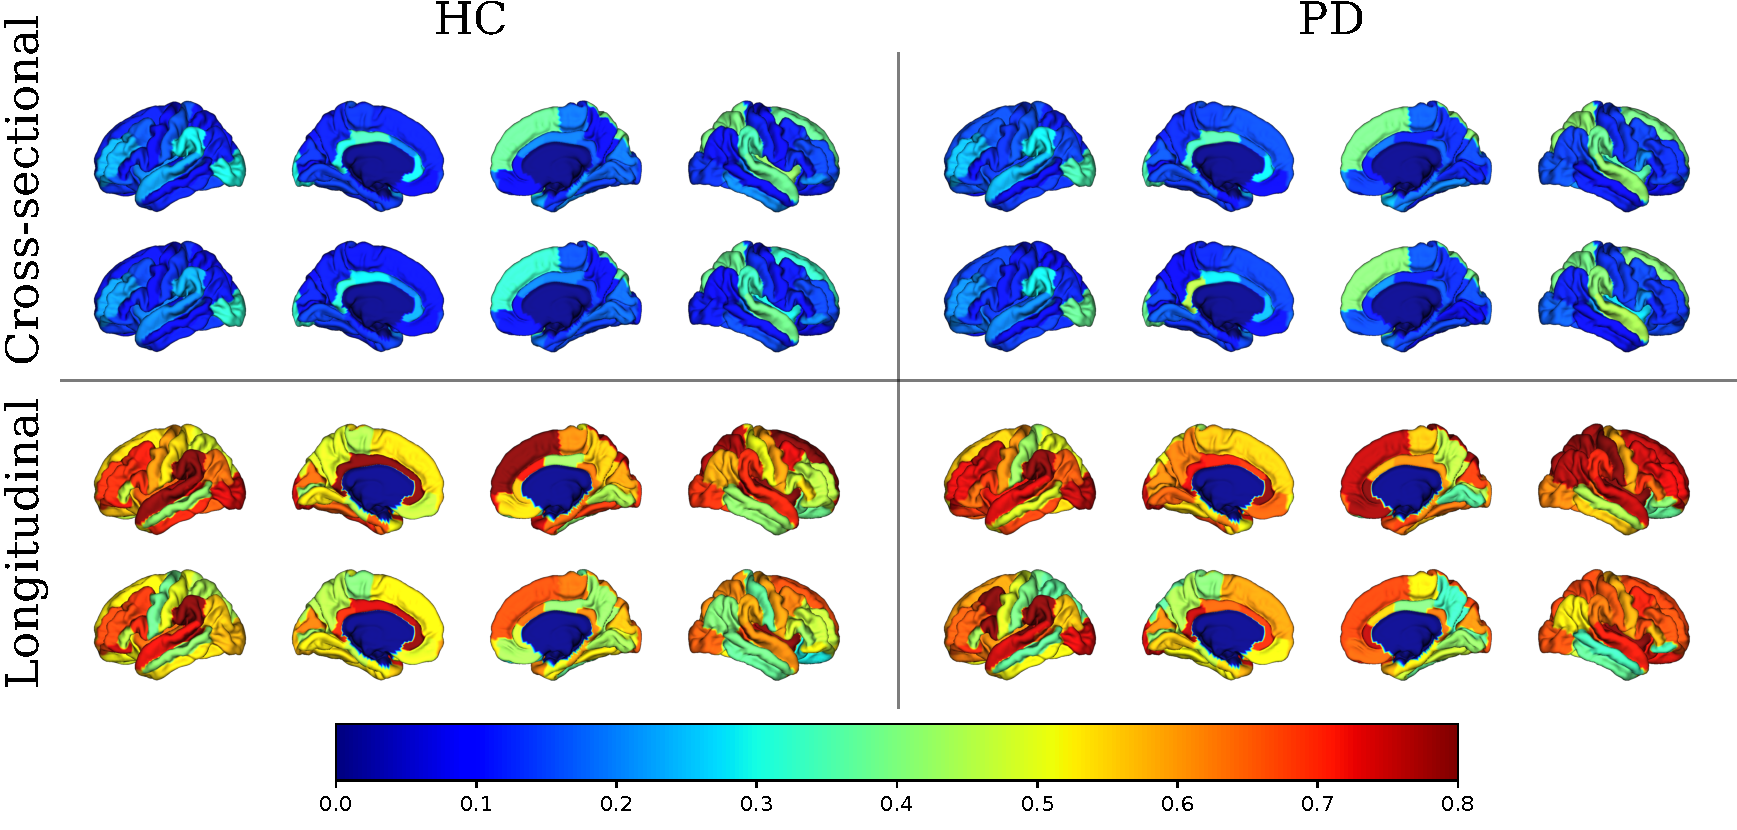
\includegraphics[width=\textwidth]{figures/NPV_map/figure_area_volume.pdf}
    \caption{Numerical-Population Variability Ratio (\navr) for cortical surface
        (top row in each panel) area and cortical volume (bottom row) in HC and
        PD. Panels show \navr{} maps at baseline for PD (a) and (HC),
        longitudinally for HC (c) and PD (d). Higher \navr{} values indicate
        greater computational uncertainty relative to inter-subject anatomical
        variability. Warmer colors denote higher \navr{} values.}
    \label{fig:navr_maps_area_volume}
\end{figure}

\subsection{Consistency results}

We evaluated the stability of statistical inferences by quantifying the
frequency of significance flipping across 26 MCA repetitions
(Table~\ref{tab:fluctuating_regions}). The analysis revealed that longitudinal
processing introduces considerably more instability than baseline
cross-sectional analysis, particularly for cortical metrics. Notably, partial
correlation analysis exhibited higher susceptibility to instability in cortical
volume (53\% of regions unstable) and area (38\% unstable) compared to ANCOVA.

To investigate whether longitudinal processing amplifies numerical instability,
we compared the dispersion of the test statistics ($F$-values for ANCOVA,
correlation coefficients $r$ for partial correlation) in longitudinal versus
cross-sectional pipelines. We used a one-sided Ansari-Bradley test on
mean-centered distributions to test the specific hypothesis that longitudinal
processing significantly has higher numerical variance compared to the baseline
(Tables~\ref{tab:stats-coef-var-subcortical} and
\ref{tab:stats-coef-var-cortical}).

For subcortical structures (Table~\ref{tab:stats-coef-var-subcortical}), partial
correlation yielded significantly higher variance in the longitudinal setting
for nearly all regions (13/14), whereas ANCOVA remained largely stable, with
only the caudate showing significant variance inflation. This trend was mirrored
in cortical regions (Table~\ref{tab:stats-coef-var-cortical}); partial
correlation analysis consistently demonstrated significantly greater variance
longitudinally across volume, thickness, and surface area. In contrast, ANCOVA
showed significant variance differences in far fewer regions.

\begin{table}[ht]
    \centering
    \small
    \setlength{\tabcolsep}{6pt}
    \renewcommand{\arraystretch}{1.15}
    \caption{Variance variability in subcortical structures
        (Ansari-Bradley test). Comparison of cross-sectional vs. longitudinal
        variances of test statistics. Significant results (*) indicate that
        longitudinal variance is significantly greater than baseline variance
        ($p_{\text{FDR}} < 0.05$, one-sided). $W$: test statistic.}
    \label{tab:fluctuating_regions}
    \begin{tabular}{lcccc}
        \hline
        \multirow{2}{*}{\textbf{Metric}}    &
        \multicolumn{2}{c}{\textbf{ANCOVA}} &
        \multicolumn{2}{c}{\textbf{Partial correlation}}                                                                            \\
        \cline{2-5}
                                            & \textbf{Baseline} & \textbf{Longitudinal} & \textbf{Baseline} & \textbf{Longitudinal} \\
        \hline
        Cortical Area (68 regions)          & 18 (27\%)         & 36 (53\%)             & 4 (6\%)           & 26 (38\%)             \\
        Cortical Thickness (68 regions)     & 11 (16\%)         & 9 (13\%)              & 19 (28\%)         & 17 (25\%)             \\
        Cortical Volume (68 regions)        & 14 (20\%)         & 20 (29\%)             & 8 (12\%)          & 36 (53\%)             \\
        Subcortical Volume (14 regions)     & 4 (29\%)          & 2 (14\%)              & 4 (29\%)          & 5 (36\%)              \\
        \hline
    \end{tabular}
\end{table}

% Table 1: Subcortical Structures
\begin{table}[h]
    \centering
    \centering
    \caption={Variance variability in cortical regions. One-sided
    Ansari-Bradley test comparing cross-sectional vs. longitudinal variances of
    test statistics. ($* p_{\text{FDR}} < 0.05$). L/R =
    Left/Right.  $W$ = statistic, $p$ = p-value.}
    \label{tab:stats-coef-var-subcortical}
    \begin{tblr}[
        ]
        {
            width = \textwidth,
            colspec = {l | Q[c,m] Q[c,m] | Q[c,m] Q[c,m]},
            row{odd} = {gray9},
            row{even} = {white},
            row{1} = {font=\bfseries, white},
            row{2} = {font=\bfseries, gray9},
            rows = {rowsep=0pt},
            rowhead = 2,
        }
        \hline
        \SetCell[r=2]{m} Region & \SetCell[c=2]{c} ANCOVA &          & \SetCell[c=2]{c} Partial Corr &         \\
        \hline
                                & W                       & p        & W                             & p       \\
        \hline
        L-Thalamus              & 248                     & 1.00     & 465                           & 6.1e-6* \\
        L-Caudate               & 501                     & 3.1e-10* & 459                           & 2.0e-5* \\
        L-Putamen               & 327                     & 0.81     & 491                           & 9.6e-9* \\
        L-Pallidum              & 264                     & 1.00     & 449                           & 1.1e-4* \\
        L-Hippocampus           & 314                     & 0.91     & 428                           & 2.2e-3* \\
        L-Amygdala              & 261                     & 1.00     & 476                           & 5.5e-7* \\
        L-Accumbens             & 265                     & 1.00     & 442                           & 3.3e-4* \\
        R-Thalamus              & 281                     & 1.00     & 441                           & 3.9e-4* \\
        R-Caudate               & 485                     & 5.5e-8*  & 478                           & 3.4e-7* \\
        R-Putamen               & 294                     & 0.98     & 489                           & 1.7e-8* \\
        R-Pallidum              & 212                     & 1.00     & 469                           & 2.7e-6* \\
        R-Hippocampus           & 335                     & 0.73     & 493                           & 5.1e-9* \\
        R-Amygdala              & 316                     & 0.90     & 408                           & 1.9e-2* \\
        R-Accumbens             & 214                     & 1.00     & 418                           & 7.0e-3* \\
        \hline
    \end{tblr}
\end{table}

% Table 2: Cortical Regions
\begin{longtblr}[
        caption={Ansari-Bradley test results for cross-sectional vs. longitudinal variances in cortical regions. * indicates FDR-corrected significance ($p < 0.05$). lh/rh =
                left/right hemisphere. ACC = anterior cingulate cortex, MF = middle
                frontal. $W$ = statistic, $p$ = p-value.},
        label={tab:stats-coef-var-cortical},
    ]{
        width=\linewidth,
        colspec = {l | *{4}{Q[c,m]} | *{4}{Q[c,m]} | *{4}{Q[c,m]}},
        row{odd} = {gray9},
        row{even} = {white},
        row{1} = {font=\bfseries, white},
        row{2} = {font=\bfseries, gray9},
        row{3} = {font=\bfseries, white},
        rows = {font=\footnotesize, rowsep=0pt},
        rowhead = 3,
    }
    \hline
    \SetCell[r=3]{m} Region   & \SetCell[c=4]{c} Cortical Volume &          &                               &          & \SetCell[c=4]{c} Cortical Thickness &          &                               &         & \SetCell[c=4]{c} Cortical Area &          &                               &          \\
    \hline
                              & \SetCell[c=2]{c} ANCOVA          &          & \SetCell[c=2]{c} Partial Corr &          & \SetCell[c=2]{c} ANCOVA             &          & \SetCell[c=2]{c} Partial Corr &         & \SetCell[c=2]{c} ANCOVA        &          & \SetCell[c=2]{c} Partial Corr &          \\
    \hline
                              & W                                & p        & W                             & p        & W                                   & p        & W                             & p       & W                              & p        & W                             & p        \\
    \hline
    bankssts (lh)             & 447                              & 1.6e-4*  & 486                           & 4.1e-8*  & 454                                 & 4.8e-5*  & 433                           & 1.2e-3* & 455                            & 4.1e-5*  & 481                           & 1.6e-7*  \\
    bankssts (rh)             & 403                              & 2.9e-2   & 466                           & 5.0e-6*  & 469                                 & 2.7e-6*  & 449                           & 1.1e-4* & 447                            & 1.6e-4*  & 461                           & 1.3e-5*  \\
    caudalACC (lh)            & 446                              & 1.8e-4*  & 487                           & 3.1e-8*  & 322                                 & 0.86     & 475                           & 6.9e-7* & 350                            & 0.52     & 480                           & 2.0e-7*  \\
    caudalACC (rh)            & 327                              & 0.81     & 513                           & 1.1e-12* & 501                                 & 3.1e-10* & 453                           & 5.8e-5* & 304                            & 0.96     & 500                           & 4.6e-10* \\
    caudalMF (lh)             & 437                              & 6.8e-4*  & 420                           & 5.6e-3*  & 479                                 & 2.6e-7*  & 413                           & 1.2e-2  & 362                            & 0.35     & 461                           & 1.3e-5*  \\
    caudalMF (rh)             & 439                              & 5.2e-4*  & 479                           & 2.6e-7*  & 352                                 & 0.49     & 445                           & 2.1e-4* & 390                            & 8.0e-2   & 489                           & 1.7e-8*  \\
    cuneus (lh)               & 441                              & 3.9e-4*  & 471                           & 1.7e-6*  & 507                                 & 2.6e-11* & 454                           & 4.8e-5* & 486                            & 4.1e-8*  & 483                           & 9.4e-8*  \\
    cuneus (rh)               & 387                              & 9.8e-2   & 481                           & 1.6e-7*  & 474                                 & 8.7e-7*  & 461                           & 1.3e-5* & 497                            & 1.4e-9*  & 487                           & 3.1e-8*  \\
    entorhinal (lh)           & 359                              & 0.39     & 409                           & 1.7e-2   & 297                                 & 0.98     & 396                           & 5.2e-2  & 474                            & 8.7e-7*  & 434                           & 1.0e-3*  \\
    entorhinal (rh)           & 372                              & 0.23     & 428                           & 2.2e-3*  & 246                                 & 1.00     & 396                           & 5.2e-2  & 505                            & 6.2e-11* & 455                           & 4.1e-5*  \\
    fusiform (lh)             & 477                              & 4.3e-7*  & 447                           & 1.6e-4*  & 421                                 & 5.0e-3*  & 419                           & 6.3e-3* & 421                            & 5.0e-3*  & 455                           & 4.1e-5*  \\
    fusiform (rh)             & 457                              & 2.8e-5*  & 460                           & 1.6e-5*  & 423                                 & 4.0e-3*  & 437                           & 6.8e-4* & 475                            & 6.9e-7*  & 454                           & 4.8e-5*  \\
    inferiorparietal (lh)     & 477                              & 4.3e-7*  & 503                           & 1.4e-10* & 347                                 & 0.56     & 458                           & 2.4e-5* & 487                            & 3.1e-8*  & 471                           & 1.7e-6*  \\
    inferiorparietal (rh)     & 369                              & 0.26     & 427                           & 2.5e-3*  & 460                                 & 1.6e-5*  & 383                           & 0.13    & 409                            & 1.7e-2   & 455                           & 4.1e-5*  \\
    inferiortemporal (lh)     & 437                              & 6.8e-4*  & 444                           & 2.5e-4*  & 356                                 & 0.44     & 461                           & 1.3e-5* & 472                            & 1.4e-6*  & 444                           & 2.5e-4*  \\
    inferiortemporal (rh)     & 335                              & 0.73     & 406                           & 2.3e-2   & 326                                 & 0.82     & 457                           & 2.8e-5* & 375                            & 0.20     & 456                           & 3.4e-5*  \\
    isthmuscingulate (lh)     & 432                              & 1.3e-3*  & 504                           & 9.5e-11* & 515                                 & 3.1e-13* & 462                           & 1.1e-5* & 413                            & 1.2e-2   & 505                           & 6.2e-11* \\
    isthmuscingulate (rh)     & 494                              & 3.7e-9*  & 469                           & 2.7e-6*  & 489                                 & 1.7e-8*  & 455                           & 4.1e-5* & 513                            & 1.1e-12* & 474                           & 8.7e-7*  \\
    lateraloccipital (lh)     & 494                              & 3.7e-9*  & 470                           & 2.1e-6*  & 430                                 & 1.7e-3*  & 440                           & 4.5e-4* & 475                            & 6.9e-7*  & 460                           & 1.6e-5*  \\
    lateraloccipital (rh)     & 472                              & 1.4e-6*  & 454                           & 4.8e-5*  & 498                                 & 9.5e-10* & 412                           & 1.3e-2  & 471                            & 1.7e-6*  & 461                           & 1.3e-5*  \\
    lateralorbitofrontal (lh) & 265                              & 1.00     & 414                           & 1.1e-2   & 184                                 & 1.00     & 464                           & 7.5e-6* & 294                            & 0.98     & 440                           & 4.5e-4*  \\
    lateralorbitofrontal (rh) & 271                              & 1.00     & 478                           & 3.4e-7*  & 422                                 & 4.5e-3*  & 429                           & 2.0e-3* & 258                            & 1.00     & 468                           & 3.3e-6*  \\
    lingual (lh)              & 250                              & 1.00     & 463                           & 9.1e-6*  & 494                                 & 3.7e-9*  & 468                           & 3.3e-6* & 453                            & 5.8e-5*  & 497                           & 1.4e-9*  \\
    lingual (rh)              & 435                              & 9.0e-4*  & 460                           & 1.6e-5*  & 480                                 & 2.0e-7*  & 467                           & 4.1e-6* & 477                            & 4.3e-7*  & 459                           & 2.0e-5*  \\
    medialorbitofrontal (lh)  & 459                              & 2.0e-5*  & 467                           & 4.1e-6*  & 479                                 & 2.6e-7*  & 410                           & 1.6e-2  & 396                            & 5.2e-2   & 469                           & 2.7e-6*  \\
    medialorbitofrontal (rh)  & 395                              & 5.6e-2   & 484                           & 7.2e-8*  & 300                                 & 0.97     & 430                           & 1.7e-3* & 405                            & 2.5e-2   & 459                           & 2.0e-5*  \\
    middletemporal (lh)       & 488                              & 2.3e-8*  & 487                           & 3.1e-8*  & 252                                 & 1.00     & 419                           & 6.3e-3* & 457                            & 2.8e-5*  & 464                           & 7.5e-6*  \\
    middletemporal (rh)       & 352                              & 0.49     & 463                           & 9.1e-6*  & 396                                 & 5.2e-2   & 428                           & 2.2e-3* & 427                            & 2.5e-3*  & 450                           & 9.5e-5*  \\
    parahippocampal (lh)      & 502                              & 2.1e-10* & 476                           & 5.5e-7*  & 462                                 & 1.1e-5*  & 437                           & 6.8e-4* & 425                            & 3.2e-3*  & 463                           & 9.1e-6*  \\
    parahippocampal (rh)      & 473                              & 1.1e-6*  & 468                           & 3.3e-6*  & 349                                 & 0.54     & 458                           & 2.4e-5* & 415                            & 9.6e-3*  & 459                           & 2.0e-5*  \\
    paracentral (lh)          & 314                              & 0.91     & 424                           & 3.6e-3*  & 204                                 & 1.00     & 425                           & 3.2e-3* & 491                            & 9.6e-9*  & 438                           & 6.0e-4*  \\
    paracentral (rh)          & 331                              & 0.77     & 484                           & 7.2e-8*  & 280                                 & 1.00     & 441                           & 3.9e-4* & 330                            & 0.78     & 485                           & 5.5e-8*  \\
    parsopercularis (lh)      & 362                              & 0.35     & 461                           & 1.3e-5*  & 494                                 & 3.7e-9*  & 418                           & 7.0e-3* & 459                            & 2.0e-5*  & 472                           & 1.4e-6*  \\
    parsopercularis (rh)      & 388                              & 9.1e-2   & 482                           & 1.2e-7*  & 305                                 & 0.96     & 477                           & 4.3e-7* & 447                            & 1.6e-4*  & 466                           & 5.0e-6*  \\
    parsorbitalis (lh)        & 293                              & 0.98     & 490                           & 1.3e-8*  & 230                                 & 1.00     & 462                           & 1.1e-5* & 419                            & 6.3e-3*  & 462                           & 1.1e-5*  \\
    parsorbitalis (rh)        & 295                              & 0.98     & 455                           & 4.1e-5*  & 336                                 & 0.71     & 427                           & 2.5e-3* & 269                            & 1.00     & 471                           & 1.7e-6*  \\
    parstriangularis (lh)     & 339                              & 0.68     & 507                           & 2.6e-11* & 401                                 & 3.5e-2   & 419                           & 6.3e-3* & 419                            & 6.3e-3*  & 504                           & 9.5e-11* \\
    parstriangularis (rh)     & 404                              & 2.7e-2   & 455                           & 4.1e-5*  & 288                                 & 0.99     & 394                           & 6.0e-2  & 362                            & 0.35     & 463                           & 9.1e-6*  \\
    pericalcarine (lh)        & 442                              & 3.3e-4*  & 465                           & 6.1e-6*  & 441                                 & 3.9e-4*  & 470                           & 2.1e-6* & 460                            & 1.6e-5*  & 509                           & 9.9e-12* \\
    pericalcarine (rh)        & 390                              & 8.0e-2   & 449                           & 1.1e-4*  & 480                                 & 2.0e-7*  & 451                           & 8.1e-5* & 443                            & 2.9e-4*  & 492                           & 7.0e-9*  \\
    postcentral (lh)          & 329                              & 0.79     & 460                           & 1.6e-5*  & 331                                 & 0.77     & 423                           & 4.0e-3* & 372                            & 0.23     & 477                           & 4.3e-7*  \\
    postcentral (rh)          & 350                              & 0.52     & 449                           & 1.1e-4*  & 269                                 & 1.00     & 426                           & 2.8e-3* & 514                            & 6.1e-13* & 387                           & 9.8e-2   \\
    posteriorcingulate (lh)   & 317                              & 0.90     & 488                           & 2.3e-8*  & 487                                 & 3.1e-8*  & 436                           & 7.9e-4* & 328                            & 0.80     & 465                           & 6.1e-6*  \\
    posteriorcingulate (rh)   & 315                              & 0.91     & 478                           & 3.4e-7*  & 480                                 & 2.0e-7*  & 450                           & 9.5e-5* & 356                            & 0.44     & 485                           & 5.5e-8*  \\
    precentral (lh)           & 284                              & 0.99     & 457                           & 2.8e-5*  & 239                                 & 1.00     & 372                           & 0.23    & 444                            & 2.5e-4*  & 424                           & 3.6e-3*  \\
    precentral (rh)           & 325                              & 0.83     & 420                           & 5.6e-3*  & 312                                 & 0.93     & 387                           & 9.8e-2  & 470                            & 2.1e-6*  & 488                           & 2.3e-8*  \\
    precuneus (lh)            & 240                              & 1.00     & 408                           & 1.9e-2   & 251                                 & 1.00     & 483                           & 9.4e-8* & 410                            & 1.6e-2   & 430                           & 1.7e-3*  \\
    precuneus (rh)            & 288                              & 0.99     & 414                           & 1.1e-2   & 244                                 & 1.00     & 465                           & 6.1e-6* & 363                            & 0.34     & 457                           & 2.8e-5*  \\
    rostralACC (lh)           & 269                              & 1.00     & 436                           & 7.9e-4*  & 505                                 & 6.2e-11* & 467                           & 4.1e-6* & 353                            & 0.48     & 460                           & 1.6e-5*  \\
    rostralACC (rh)           & 275                              & 1.00     & 501                           & 3.1e-10* & 481                                 & 1.6e-7*  & 448                           & 1.3e-4* & 275                            & 1.00     & 448                           & 1.3e-4*  \\
    rostralmiddlefrontal (lh) & 370                              & 0.25     & 482                           & 1.2e-7*  & 276                                 & 1.00     & 430                           & 1.7e-3* & 283                            & 0.99     & 489                           & 1.7e-8*  \\
    rostralmiddlefrontal (rh) & 318                              & 0.89     & 418                           & 7.0e-3*  & 319                                 & 0.88     & 431                           & 1.5e-3* & 219                            & 1.00     & 442                           & 3.3e-4*  \\
    superiorfrontal (lh)      & 370                              & 0.25     & 443                           & 2.9e-4*  & 456                                 & 3.4e-5*  & 464                           & 7.5e-6* & 481                            & 1.6e-7*  & 435                           & 9.0e-4*  \\
    superiorfrontal (rh)      & 392                              & 6.9e-2   & 432                           & 1.3e-3*  & 271                                 & 1.00     & 467                           & 4.1e-6* & 376                            & 0.19     & 480                           & 2.0e-7*  \\
    superiorparietal (lh)     & 369                              & 0.26     & 333                           & 0.75     & 369                                 & 0.26     & 440                           & 4.5e-4* & 489                            & 1.7e-8*  & 386                           & 0.10     \\
    superiorparietal (rh)     & 506                              & 4.0e-11* & 430                           & 1.7e-3*  & 437                                 & 6.8e-4*  & 463                           & 9.1e-6* & 456                            & 3.4e-5*  & 430                           & 1.7e-3*  \\
    superiortemporal (lh)     & 413                              & 1.2e-2   & 484                           & 7.2e-8*  & 427                                 & 2.5e-3*  & 441                           & 3.9e-4* & 446                            & 1.8e-4*  & 481                           & 1.6e-7*  \\
    superiortemporal (rh)     & 401                              & 3.5e-2   & 452                           & 6.8e-5*  & 364                                 & 0.32     & 469                           & 2.7e-6* & 425                            & 3.2e-3*  & 470                           & 2.1e-6*  \\
    supramarginal (lh)        & 466                              & 5.0e-6*  & 466                           & 5.0e-6*  & 274                                 & 1.00     & 488                           & 2.3e-8* & 509                            & 9.9e-12* & 481                           & 1.6e-7*  \\
    supramarginal (rh)        & 394                              & 6.0e-2   & 422                           & 4.5e-3*  & 483                                 & 9.4e-8*  & 412                           & 1.3e-2  & 376                            & 0.19     & 432                           & 1.3e-3*  \\
    frontalpole (lh)          & 385                              & 0.11     & 445                           & 2.1e-4*  & 319                                 & 0.88     & 453                           & 5.8e-5* & 347                            & 0.56     & 428                           & 2.2e-3*  \\
    frontalpole (rh)          & 284                              & 0.99     & 410                           & 1.6e-2   & 391                                 & 7.5e-2   & 451                           & 8.1e-5* & 218                            & 1.00     & 399                           & 4.1e-2   \\
    temporalpole (lh)         & 356                              & 0.44     & 379                           & 0.16     & 308                                 & 0.94     & 384                           & 0.12    & 385                            & 0.11     & 436                           & 7.9e-4*  \\
    temporalpole (rh)         & 252                              & 1.00     & 344                           & 0.61     & 421                                 & 5.0e-3*  & 403                           & 2.9e-2  & 225                            & 1.00     & 396                           & 5.2e-2   \\
    transversetemporal (lh)   & 406                              & 2.3e-2   & 467                           & 4.1e-6*  & 367                                 & 0.29     & 421                           & 5.0e-3* & 445                            & 2.1e-4*  & 482                           & 1.2e-7*  \\
    transversetemporal (rh)   & 324                              & 0.84     & 417                           & 7.8e-3*  & 477                                 & 4.3e-7*  & 442                           & 3.3e-4* & 347                            & 0.56     & 435                           & 9.0e-4*  \\
    insula (lh)               & 249                              & 1.00     & 470                           & 2.1e-6*  & 220                                 & 1.00     & 457                           & 2.8e-5* & 263                            & 1.00     & 438                           & 6.0e-4*  \\
    insula (rh)               & 267                              & 1.00     & 444                           & 2.5e-4*  & 401                                 & 3.5e-2   & 439                           & 5.2e-4* & 235                            & 1.00     & 410                           & 1.6e-2   \\
    \hline
\end{longtblr}

\begin{table}[t]
    \centering
    \caption{Permutation test comparison of $\nu_{\text{nav}}$ between HC and PD.
        No significance detected after Bonferroni correction ($\alpha=0.05/8$).
        Values are observed differences (PD$-$HC). 95\% CIs from percentile bootstrap.}
    \label{tab:bootstrap-navr}
    \begin{tabular}{lcccc}
        \toprule
        \textbf{Metric}    & {\textbf{Observed} $\Delta$} & \textbf{95\% CI}    & {\textbf{p-value}} & \textbf{Study}  \\
        \midrule
        area               & 0.005                        & {[}-0.002, 0.013{]} & 0.734              & cross-sectional \\
        thickness          & 0.027                        & {[}0.020, 0.034{]}  & 0.033              & cross-sectional \\
        volume             & 0.013                        & {[} 0.004, 0.022{]} & 0.371              & cross-sectional \\
        subcortical volume & 0.014                        & {[} 0.004, 0.025{]} & 0.646              & cross-sectional \\
        \midrule
        area               & 0.021                        & {[}-0.002, 0.044{]} & 0.482              & longitudinal    \\
        thickness          & 0.002                        & {[}-0.014, 0.020{]} & 0.919              & longitudinal    \\
        volume             & 0.025                        & {[} 0.002, 0.049{]} & 0.370              & longitudinal    \\
        subcortical volume & -0.027                       & {[}-0.047,-0.006{]} & 0.489              & longitudinal    \\
        \bottomrule
    \end{tabular}
\end{table}

\subsubsection{Consistency of statistical tests}

For both group comparisons and correlation analyses, statistical outcomes varied
substantially across the 26 Monte Carlo Arithmetic (MCA) repetitions (Figures
\ref{fig:navr_consistency_area_plot} and \ref{fig:consistency_volume_plot}). For
cortical area (68 regions; Figure \ref{fig:navr_consistency_area_plot}),
significance flipped in 31\% of all (regions, analysis) pairs, indicating
frequent inconsistencies across repetitions. For cortical volume (68 regions;
Figure \ref{fig:consistency_volume_plot}), 29\% of pairs were similarly unstable.
These fluctuations demonstrate that numerical noise alone can alter downstream
statistical inference in structural MRI analyses of PD.

\begin{figure}[h]
    \centering
    \includegraphics[width=\linewidth]{figures/consistency/cortical_area_significance_correlation.pdf}
    \caption{Consistency of statistical tests for cortical area across all
        subjects and regions. The plot shows the percentage of subjects for
        which the statistical test was significant ($\alpha = 0.05$) for each
        region. The consistency varies across regions, with some regions showing
        higher consistency than others.}
    \label{fig:navr_consistency_area_plot}
\end{figure}

\begin{figure}[h]
    \centering
    \includegraphics[width=\linewidth]{figures/consistency/cortical_volume_significance_correlation.pdf}
    \caption{Consistency of statistical tests for cortical volume across all
        subjects and regions. The plot shows the percentage of subjects for
        which the statistical test was significant ($\alpha = 0.05$) for each
        region. The consistency varies across regions, with some regions showing
        higher consistency than others.}
    \label{fig:consistency_volume_plot}
\end{figure}

\subsection{Interactive web tool}

\begin{figure}[ht]
    \centering
    \includegraphics[width=0.7\linewidth]{figures/screenshot_light.png}
    \caption{Interactive web tool for estimating NPVR and assessing numerical
        variability in neuroimaging studies. Users can input summary statistics
        to obtain NPVR values and visualize the impact of numerical variability
        on effect size estimates. The tool is available at
        \href{https://yohanchatelain.github.io/brain\_render/}{yohanchatelain.github.io/brain\_render}.
        \label{fig:brain_render_tool}}
\end{figure}

\section{Distribution of statistical tests coefficients}
\label{appendix:distribution_stats_ieee}

Figures \ref{fig:statstest_coefficients_distribution},
\ref{fig:consistency_area_coefficients} and
\ref{fig:consistency_volume_coefficients} show the distribution of partial
correlation coefficients and F-statistics for subcortical volume measures,
cortical thickness, cortical areas and cortical volumes, across all subjects
and regions. Red triangles indicate the unperturbed (IEEE-754) run for
reference. For all analyses, the unperturbed (IEEE-754) result is included in
the range of numericallly perturbed results, which supports the validity of the
numerical perturbation.

% The distribution shows the variability in the
% coefficients, with some regions exhibiting higher consistency than others.

% For subcortical volumes, the distributions of partial-correlation coefficients
% ($r$) and ANCOVA $F$-statistics
% (Figure~\ref{fig:statstest_coefficients_distribution}) show that the unperturbed
% IEEE-754 estimates (red markers) consistently fall within the MCA-sampled range.
% This supports the validity of the instrumentation rather than indicating a
% methodological artifact. The spread of the $r$ coefficients is larger in
% longitudinal than in baseline analyses (Ansari-Bradley one-sided test at
% $p<0.05$ corrected with Bonferroni; detailed results in Appendix
% Table~\ref{tab:stats-coef-var-subcortical}), whereas no significant difference
% in spread is detected for $F$-statistics using the same test
% (Bonferroni-corrected, $p<0.05$). This indicates that numerical variability has
% a more pronounced impact on longitudinal studies than on cross-sectional ones.
% An analogous analysis for cortical thickness leads to similar conclusions
% (Appendix Figure~\ref{fig:consistency_thickness_coefficients},
% Table~\ref{tab:stats-coef-var-cortical}).

\begin{figure}[ht]
    \centering
    \includegraphics[width=\linewidth]{figures/consistency/subcortical_volume_coefficients_distribution.pdf}
    \caption{ Distribution of partial correlation coefficients (r-values) and
        F-statistics from ANCOVA across MCA repetitions for subcortical volume
        measures. Red dots represent the IEEE-754 unperturbed results.
        \label{fig:statstest_coefficients_distribution}}
\end{figure}

\begin{figure}
    \centering
    \begin{subfigure}[b]{\linewidth}
        \centering
        \includegraphics[width=.9\linewidth]{figures/consistency/cortical_thickness_coefficients_distribution-Left.pdf}
        \caption{Left hemisphere}
        \label{fig:consistency_thickness_left}
    \end{subfigure}

    \begin{subfigure}[b]{\linewidth}
        \centering
        \includegraphics[width=.9\linewidth]{figures/consistency/cortical_thickness_coefficients_distribution-Right.pdf}
        \caption{Right hemisphere}
        \label{fig:consistency_thickness_right}
    \end{subfigure}
    \caption{Distribution of partial correlation coefficients for cortical
        thickness across all subjects and regions. Red triangles indicate the
        IEEE-754 run for reference. }
    \label{fig:consistency_thickness_coefficients}
\end{figure}

\begin{figure}[h]
    \centering
    \begin{subfigure}[b]{\linewidth}
        \centering
        \includegraphics[width=.9\linewidth]{figures/consistency/cortical_area_coefficients_distribution-Left.pdf}
        \caption{Left hemisphere}
        \label{fig:consistency_area_left}
    \end{subfigure}
    \hfill
    \begin{subfigure}[b]{\linewidth}
        \centering
        \includegraphics[width=.9\linewidth]{figures/consistency/cortical_area_coefficients_distribution-Right.pdf}
        \caption{Right hemisphere}
        \label{fig:consistency_area_right}
    \end{subfigure}
    \caption{ Distribution of partial correlation coefficients for cortical surface area
        across all subjects and regions. Red triangles indicate the IEEE-754 run
        for reference. }
    \label{fig:consistency_area_coefficients}
\end{figure}

\begin{figure}[h]
    \centering
    \begin{subfigure}[b]{\linewidth}
        \centering
        \includegraphics[width=.9\linewidth]{figures/consistency/cortical_volume_coefficients_distribution-Left.pdf}
        \caption{Left hemisphere}
        \label{fig:consistency_volume_left}
    \end{subfigure}
    \hfill
    \begin{subfigure}[b]{\linewidth}
        \centering
        \includegraphics[width=.9\linewidth]{figures/consistency/cortical_volume_coefficients_distribution-Right.pdf}
        \caption{Right hemisphere}
        \label{fig:consistency_volume_right}
    \end{subfigure}
    \caption{ Distribution of partial correlation coefficients for cortical
        volume across all subjects and regions. Red triangles indicate the
        IEEE-754 run for reference. The distribution shows the variability in
        the coefficients, with some regions exhibiting higher consistency than
        others.}
    \label{fig:consistency_volume_coefficients}
\end{figure}

\begin{figure}[h]
    \centering
    \vspace{0.2cm}

    % Header row with column labels
    \begin{minipage}[b]{\linewidth}
        \begin{minipage}[c]{0.05\linewidth}
            % Empty space for alignment with condition labels
        \end{minipage}%
        \begin{minipage}[c]{0.95\linewidth}
            \begin{minipage}[c]{0.47\linewidth}
                \centering\textbf{Unthresholded}
            \end{minipage}%
            \hfill
            \begin{minipage}[c]{0.005\linewidth}
                % Vertical line separator
            \end{minipage}%
            \hfill
            \begin{minipage}[c]{0.47\linewidth}
                \centering\textbf{Thresholded}
            \end{minipage}
        \end{minipage}
    \end{minipage}

    % Horizontal line
    \noindent\rule{\linewidth}{0.5pt}
    \vspace{-1.5cm}

    % 22q11.2 deletion syndrome row
    \begin{minipage}[b]{\linewidth}
        \begin{minipage}[c]{0.05\linewidth}
            \centering\rotatebox{90}{\textbf{22q11.2}} \end{minipage}%
        \begin{minipage}[c]{0.95\linewidth}
            \begin{subfigure}[c]{0.47\linewidth}
                \includegraphics[width=\linewidth]{figures/cohen_d_map/enigma/22q_area_all.png}
                \label{fig:enigma_22q_unthresholded}
            \end{subfigure}%
            \hfill
            \begin{minipage}[c]{0.005\linewidth}
                \centering\rule{0.5pt}{4cm}
            \end{minipage}%
            \hfill
            \begin{subfigure}[c]{0.47\linewidth}
                \includegraphics[width=\linewidth]{figures/cohen_d_map/enigma/22q_area_all_thresholded.png}
                \label{fig:enigma_22q_thresholded}
            \end{subfigure}
        \end{minipage}
    \end{minipage}

    \vspace{-2cm}

    % ADHD row
    \begin{minipage}[b]{\linewidth}
        \begin{minipage}[c]{0.05\linewidth}
            \centering\rotatebox{90}{\textbf{ADHD}} \end{minipage}%
        \begin{minipage}[c]{0.95\linewidth}
            \begin{subfigure}[c]{0.47\linewidth}
                \includegraphics[width=\linewidth]{figures/cohen_d_map/enigma/adhd_area_adult.png}
                \label{fig:enigma_adhd_unthresholded}
            \end{subfigure}%
            \hfill
            \begin{minipage}[c]{0.005\linewidth}
                \centering\rule{0.5pt}{4cm}
            \end{minipage}%
            \hfill
            \begin{subfigure}[c]{0.47\linewidth}
                \includegraphics[width=\linewidth]{figures/cohen_d_map/enigma/adhd_area_adult_thresholded.png}
                \label{fig:enigma_adhd_thresholded}
            \end{subfigure}
        \end{minipage}
    \end{minipage}

    \vspace{-2cm}

    % bipolar disorder row
    \begin{minipage}[b]{\linewidth}
        \begin{minipage}[c]{0.05\linewidth}
            \centering\rotatebox{90}{\textbf{Bipolar}} \end{minipage}%
        \begin{minipage}[c]{0.95\linewidth}
            \begin{subfigure}[c]{0.47\linewidth}
                \includegraphics[width=\linewidth]{figures/cohen_d_map/enigma/bipolar_area_adult.png}
                \label{fig:enigma_bipolar_unthresholded}
            \end{subfigure}%
            \hfill
            \begin{minipage}[c]{0.005\linewidth}
                \centering\rule{0.5pt}{4cm}
            \end{minipage}%
            \hfill
            \begin{subfigure}[c]{0.47\linewidth}
                \includegraphics[width=\linewidth]{figures/cohen_d_map/enigma/bipolar_area_adult_thresholded.png}
                \label{fig:enigma_bipolar_thresholded}
            \end{subfigure}
        \end{minipage}
    \end{minipage}

    \vspace{-2cm}
    % depression
    \begin{minipage}[b]{\linewidth}
        \begin{minipage}[c]{0.05\linewidth}
            \centering\rotatebox{90}{\textbf{Depression}} \end{minipage}%
        \begin{minipage}[c]{0.95\linewidth}
            \begin{subfigure}[c]{0.47\linewidth}
                \includegraphics[width=\linewidth]{figures/cohen_d_map/enigma/depression_area_adult.png}
                \label{fig:enigma_depression_unthresholded}
            \end{subfigure}%
            \hfill
            \begin{minipage}[c]{0.005\linewidth}
                \centering\rule{0.5pt}{4cm}
            \end{minipage}%
            \hfill
            \begin{subfigure}[c]{0.47\linewidth}
                \includegraphics[width=\linewidth]{figures/cohen_d_map/enigma/depression_area_adult_thresholded.png}
                \label{fig:enigma_depression_thresholded}
            \end{subfigure}
        \end{minipage}
    \end{minipage}

    \vspace{-2cm}
    % ocd 
    \begin{minipage}[b]{\linewidth}
        \begin{minipage}[c]{0.05\linewidth}
            \centering\rotatebox{90}{\textbf{OCD}} \end{minipage}%
        \begin{minipage}[c]{0.95\linewidth}
            \begin{subfigure}[c]{0.47\linewidth}
                \includegraphics[width=\linewidth]{figures/cohen_d_map/enigma/ocd_area_adult.png}
                \label{fig:enigma_ocd_unthresholded}
            \end{subfigure}%
            \hfill
            \begin{minipage}[c]{0.005\linewidth}
                \centering\rule{0.5pt}{4cm}
            \end{minipage}%
            \hfill
            \begin{subfigure}[c]{0.47\linewidth}
                \includegraphics[width=\linewidth]{figures/cohen_d_map/enigma/ocd_area_adult_thresholded.png}
                \label{fig:enigma_ocd_thresholded}
            \end{subfigure}
        \end{minipage}
    \end{minipage}

    \vspace{-2cm}
    % schizophrenia
    \begin{minipage}[b]{\linewidth}
        \begin{minipage}[c]{0.05\linewidth}
            \centering\rotatebox{90}{\textbf{Schizophrenia}} \end{minipage}%
        \begin{minipage}[c]{0.95\linewidth}
            \begin{subfigure}[c]{0.47\linewidth}
                \includegraphics[width=\linewidth]{figures/cohen_d_map/enigma/schizophrenia_area_all.png}
                \label{fig:enigma_schizophrenia_unthresholded}
            \end{subfigure}%
            \hfill
            \begin{minipage}[c]{0.005\linewidth}
                \centering\rule{0.5pt}{4cm}
            \end{minipage}%
            \hfill
            \begin{subfigure}[c]{0.47\linewidth}
                \includegraphics[width=\linewidth]{figures/cohen_d_map/enigma/schizophrenia_area_all_thresholded.png}
                \label{fig:enigma_schizophrenia_thresholded}
            \end{subfigure}
        \end{minipage}
    \end{minipage}

    \caption{ENIGMA cortical area Cohen's d maps showing unthresholded effect
        sizes (left) and effect sizes thresholded by the \navr framework (right)
        for different disorders. Black regions indicate areas where Cohen's d
        values fall below the numerical variability threshold, demonstrating
        regions where reported effect sizes may be unreliable due to
        computational uncertainty.}
    \label{fig:navr_enigma_area}
\end{figure}

\section{Numerical validation of flip significance simulations}
\label{appendix:numerical_validation_flip_significance}

To assess the validity of the analytical uncertainty framework used to model
numerically induced significance instability, we compared simulated estimates
derived from closed-form uncertainty expressions with empirical estimates
obtained from Monte Carlo Arithmetic (MCA) repetitions. Formally, the
proportion of significant tests (positive prediction rate, PPR) is defined as:
\begin{equation}
    \text{PPR} = \frac{\text{TP} + \text{FN}}{\text{TP} + \text{FP} + \text{TN} + \text{FN}},
    \label{eq:ppr}
\end{equation}
where TP, FP, TN, and FN denote true positives, false positives, true negatives,
and false negatives, respectively.

Figure~\ref{fig:std_sampled_simulated_comparison} compares standard deviations of
$p$-values estimated directly from 26 MCA runs with those predicted by the
analytical uncertainty formulas (Table~\ref{tab:stat_uncertainty}). Each point
corresponds to a cortical or subcortical brain region. Results show close
agreement between sampled and simulated estimates, particularly in the
cross-sectional setting. In the longitudinal analyses, simulated standard
deviations tend to be slightly larger than sampled values, indicating a
conservative bias of the analytical model.

Figure~\ref{fig:ppr_simulated_comparison} evaluates how this analytical
uncertainty propagates to downstream inference by comparing the simulated
positive prediction rate (PPR; Eq.~\ref{eq:ppr}) with the empirical proportion
of significant tests observed across MCA repetitions. Cross-sectional results
closely follow the identity line, while longitudinal results show a moderate
overestimation of PPR, consistent with the conservative overestimation of
$p$-value variability observed in Fig.~\ref{fig:std_sampled_simulated_comparison}.

Finally, Figure~\ref{fig:ppr_sampled_comparison} assesses the Beta distribution
model used to translate sampled $p$-value variability into PPR estimates.
Here, PPR is computed using MCA-derived standard deviations propagated through
the Beta model (Eq.~\ref{eq:beta-params}). Both cross-sectional and longitudinal
results align closely with the identity line, supporting the suitability of the
Beta modeling framework for capturing numerically induced variability in
statistical significance.

\begin{figure}[ht]
    \centering
    \includegraphics[width=.9\linewidth]{figures/std-sampled-simulated-comparison.pdf}
    \caption{Comparison of standard deviation estimates of $p$-values obtained from
        MCA sampling and analytical simulations. Sampled estimates are computed from
        26 MCA repetitions, while simulated estimates are derived from the
        uncertainty propagation formulas reported in
        Table~\ref{tab:stat_uncertainty}. Each point corresponds to a cortical or
        subcortical brain region. The solid line denotes the identity line. Results
        show close agreement between sampled and simulated estimates, with
        cross-sectional analyses exhibiting tighter clustering than longitudinal
        analyses. In the longitudinal setting, simulated standard deviations tend to
        slightly overestimate sampled variability, indicating conservative behavior
        of the analytical uncertainty model.
        \label{fig:std_sampled_simulated_comparison}}
\end{figure}

\begin{figure}[ht]
    \centering
    \includegraphics[width=.9\linewidth]{figures/ppr_simulated.pdf}
    \caption{ Comparison between simulated positive prediction rate (PPR;
        Eq.~\ref{eq:ppr}) and the empirical proportion of significant tests
        (Section~\ref{sec:empirical_evaluation}). Simulated PPR values are computed
        using analytical uncertainty estimates derived from
        Table~\ref{tab:stat_uncertainty}. Each point represents a cortical or
        subcortical brain region, and the solid line indicates the identity line.
        Simulated PPR closely matches empirical significance rates in the
        cross-sectional setting, while longitudinal analyses show a tendency toward
        overestimation, consistent with the corresponding overestimation of
        $p$-value variability.\label{fig:ppr_simulated_comparison}}
\end{figure}

\begin{figure}[ht]
    \centering
    \includegraphics[width=.9\linewidth]{figures/ppr_sampled.pdf}
    \caption{Comparison between sampled positive prediction rate (PPR;
        Eq.~\ref{eq:ppr}) and the empirical proportion of significant tests
        (Section~\ref{sec:empirical_evaluation}). Sampled PPR values are
        computed from MCA-derived $p$-value standard deviations and propagated
        through the Beta distribution model (Eq.~\ref{eq:beta-params}). Each
        point corresponds to a cortical or subcortical brain region, and the
        solid line denotes the identity line. Both cross-sectional and
        longitudinal results align closely with the identity line, supporting
        the suitability of the Beta modeling framework for capturing numerically
        induced variability in statistical significance.
        \label{fig:ppr_sampled_comparison}}
\end{figure}